\documentclass{standalone}
\usepackage{tikz}
\usetikzlibrary{patterns, positioning}
\usepackage[sfdefault]{ClearSans} %% option 'sfdefault' activates Clear Sans as the default text font
\usepackage[T1]{fontenc}

\begin{document}
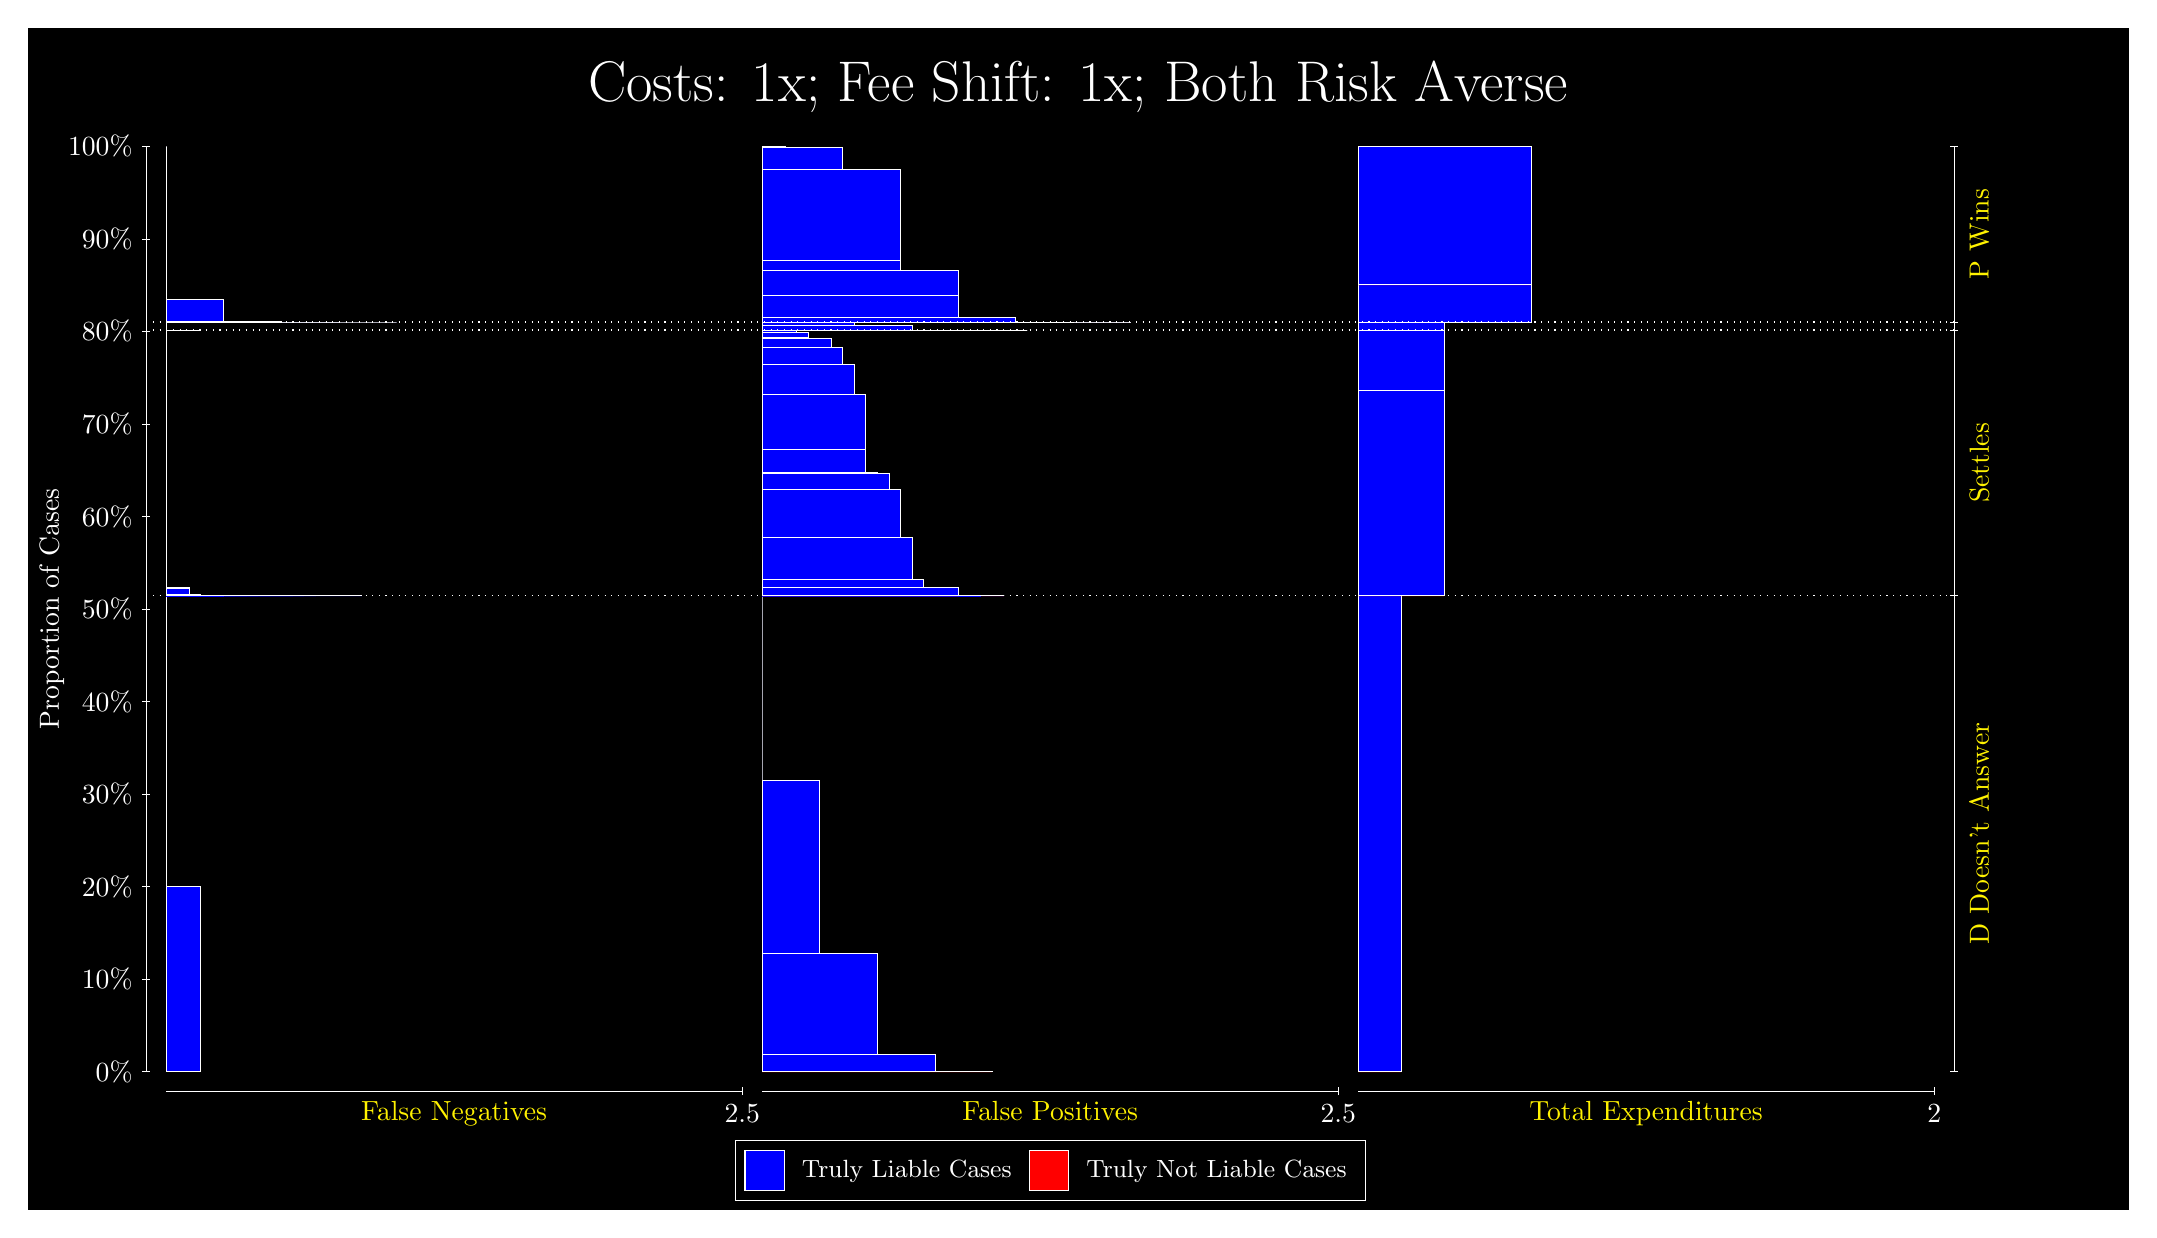
\begin{tikzpicture}
\draw[fill=black] (0,0) rectangle (26.667,15);
\draw[text=white] (0,13.5) rectangle (26.667,15) node[midway] {\huge Costs: 1x; Fee Shift: 1x; Both Risk Averse};
\draw[white, very thin] (1.5,1.75) -- (1.5,13.5);
\node[rotate=90, text=white, anchor=center] at (0.3, 7.625) {Proportion of Cases};
\draw[white, very thin] (1.45,1.75) -- (1.55,1.75);
\node[text=white, anchor=east] at (1.45, 1.75) {0\%};
\draw[white, very thin] (1.45,2.925) -- (1.55,2.925);
\node[text=white, anchor=east] at (1.45, 2.925) {10\%};
\draw[white, very thin] (1.45,4.1) -- (1.55,4.1);
\node[text=white, anchor=east] at (1.45, 4.1) {20\%};
\draw[white, very thin] (1.45,5.275) -- (1.55,5.275);
\node[text=white, anchor=east] at (1.45, 5.275) {30\%};
\draw[white, very thin] (1.45,6.45) -- (1.55,6.45);
\node[text=white, anchor=east] at (1.45, 6.45) {40\%};
\draw[white, very thin] (1.45,7.625) -- (1.55,7.625);
\node[text=white, anchor=east] at (1.45, 7.625) {50\%};
\draw[white, very thin] (1.45,8.8) -- (1.55,8.8);
\node[text=white, anchor=east] at (1.45, 8.8) {60\%};
\draw[white, very thin] (1.45,9.975) -- (1.55,9.975);
\node[text=white, anchor=east] at (1.45, 9.975) {70\%};
\draw[white, very thin] (1.45,11.15) -- (1.55,11.15);
\node[text=white, anchor=east] at (1.45, 11.15) {80\%};
\draw[white, very thin] (1.45,12.325) -- (1.55,12.325);
\node[text=white, anchor=east] at (1.45, 12.325) {90\%};
\draw[white, very thin] (1.45,13.5) -- (1.55,13.5);
\node[text=white, anchor=east] at (1.45, 13.5) {100\%};

\draw[white, very thin] (24.457,1.75) -- (24.457,13.5);
\draw[white, very thin] (24.407,1.75) -- (24.507,1.75);
\node[anchor=west] at (24.407, 1.75) {};
\draw[white, very thin] (24.407,7.7929) -- (24.507,7.7929);
\node[anchor=west] at (24.407, 7.7929) {};
\draw[white, very thin] (24.407,11.167) -- (24.507,11.167);
\node[anchor=west] at (24.407, 11.167) {};
\draw[white, very thin] (24.407,11.269) -- (24.507,11.269);
\node[anchor=west] at (24.407, 11.269) {};
\draw[white, very thin] (24.407,13.5) -- (24.507,13.5);
\node[anchor=west] at (24.407, 13.5) {};

\draw[white, very thin, fill=blue] (1.75,1.75) rectangle (2.1891,4.0983);
\draw[white, very thin, fill=red] (1.75,4.0983) rectangle (1.75,4.0983);
\draw[white, very thin, fill=blue] (1.75,4.0983) rectangle (1.75,7.7929);
\draw[white, very thin, fill=blue] (1.75,7.7929) rectangle (4.2384,7.7929);
\draw[white, very thin, fill=blue] (1.75,7.7929) rectangle (3.6529,7.7929);
\draw[white, very thin, fill=blue] (1.75,7.7929) rectangle (3.5065,7.7929);
\draw[white, very thin, fill=blue] (1.75,7.7929) rectangle (3.3602,7.7929);
\draw[white, very thin, fill=blue] (1.75,7.7929) rectangle (3.0674,7.7929);
\draw[white, very thin, fill=blue] (1.75,7.7929) rectangle (2.921,7.7929);
\draw[white, very thin, fill=blue] (1.75,7.7929) rectangle (2.7746,7.793);
\draw[white, very thin, fill=blue] (1.75,7.793) rectangle (2.6283,7.793);
\draw[white, very thin, fill=blue] (1.75,7.793) rectangle (2.4819,7.7942);
\draw[white, very thin, fill=blue] (1.75,7.7942) rectangle (2.3355,7.799);
\draw[white, very thin, fill=blue] (1.75,7.799) rectangle (2.1891,7.8156);
\draw[white, very thin, fill=blue] (1.75,7.8156) rectangle (2.0428,7.8895);
\draw[white, very thin, fill=blue] (1.75,7.8895) rectangle (2.0428,7.9015);
\draw[white, very thin, fill=blue] (1.75,7.9015) rectangle (1.8964,7.9018);
\draw[white, very thin, fill=red] (1.75,7.9018) rectangle (1.75,7.9018);
\draw[white, very thin, fill=blue] (1.75,7.9018) rectangle (1.75,11.167);
\draw[white, very thin, fill=blue] (1.75,11.167) rectangle (2.1891,11.167);
\draw[white, very thin, fill=red] (1.75,11.167) rectangle (1.75,11.167);
\draw[white, very thin, fill=blue] (1.75,11.167) rectangle (1.75,11.269);
\draw[white, very thin, fill=blue] (1.75,11.269) rectangle (4.6775,11.269);
\draw[white, very thin, fill=blue] (1.75,11.269) rectangle (3.9457,11.269);
\draw[white, very thin, fill=blue] (1.75,11.269) rectangle (3.2138,11.275);
\draw[white, very thin, fill=blue] (1.75,11.275) rectangle (2.4819,11.56);
\draw[white, very thin, fill=red] (1.75,11.56) rectangle (1.75,11.56);
\draw[white, very thin, fill=blue] (1.75,11.56) rectangle (1.75,13.5);
\draw[white, very thin, fill=red] (9.3189,1.75) rectangle (12.246,1.75);
\draw[white, very thin, fill=blue] (9.3189,1.75) rectangle (12.246,1.7522);
\draw[white, very thin, fill=blue] (9.3189,1.7522) rectangle (11.515,1.9668);
\draw[white, very thin, fill=blue] (9.3189,1.9668) rectangle (10.783,3.2564);
\draw[white, very thin, fill=blue] (9.3189,3.2564) rectangle (10.051,5.4446);
\draw[white, very thin, fill=blue] (9.3189,5.4446) rectangle (9.3189,7.7929);
\draw[white, very thin, fill=red] (9.3189,7.7929) rectangle (12.393,7.7929);
\draw[white, very thin, fill=blue] (9.3189,7.7929) rectangle (12.393,7.7929);
\draw[white, very thin, fill=red] (9.3189,7.7929) rectangle (12.1,7.7929);
\draw[white, very thin, fill=blue] (9.3189,7.7929) rectangle (12.1,7.7936);
\draw[white, very thin, fill=red] (9.3189,7.7936) rectangle (11.807,7.7936);
\draw[white, very thin, fill=blue] (9.3189,7.7936) rectangle (11.807,7.8983);
\draw[white, very thin, fill=blue] (9.3189,7.8983) rectangle (11.661,7.9051);
\draw[white, very thin, fill=red] (9.3189,7.9051) rectangle (11.515,7.9051);
\draw[white, very thin, fill=blue] (9.3189,7.9051) rectangle (11.515,7.9056);
\draw[white, very thin, fill=blue] (9.3189,7.9056) rectangle (11.368,7.9996);
\draw[white, very thin, fill=red] (9.3189,7.9996) rectangle (11.222,7.9996);
\draw[white, very thin, fill=blue] (9.3189,7.9996) rectangle (11.222,8.5396);
\draw[white, very thin, fill=blue] (9.3189,8.5396) rectangle (11.075,9.144);
\draw[white, very thin, fill=blue] (9.3189,9.144) rectangle (10.929,9.3513);
\draw[white, very thin, fill=blue] (9.3189,9.3513) rectangle (10.783,9.3598);
\draw[white, very thin, fill=blue] (9.3189,9.3598) rectangle (10.636,9.6554);
\draw[white, very thin, fill=red] (9.3189,9.6554) rectangle (10.636,9.6554);
\draw[white, very thin, fill=blue] (9.3189,9.6554) rectangle (10.636,10.346);
\draw[white, very thin, fill=blue] (9.3189,10.346) rectangle (10.49,10.737);
\draw[white, very thin, fill=blue] (9.3189,10.737) rectangle (10.344,10.951);
\draw[white, very thin, fill=blue] (9.3189,10.951) rectangle (10.197,11.058);
\draw[white, very thin, fill=blue] (9.3189,11.058) rectangle (10.051,11.058);
\draw[white, very thin, fill=blue] (9.3189,11.058) rectangle (9.9044,11.07);
\draw[white, very thin, fill=blue] (9.3189,11.07) rectangle (9.9044,11.144);
\draw[white, very thin, fill=blue] (9.3189,11.144) rectangle (9.758,11.16);
\draw[white, very thin, fill=blue] (9.3189,11.16) rectangle (9.6116,11.165);
\draw[white, very thin, fill=blue] (9.3189,11.165) rectangle (9.4652,11.166);
\draw[white, very thin, fill=blue] (9.3189,11.166) rectangle (9.3189,11.167);
\draw[white, very thin, fill=red] (9.3189,11.167) rectangle (12.686,11.167);
\draw[white, very thin, fill=blue] (9.3189,11.167) rectangle (12.686,11.167);
\draw[white, very thin, fill=blue] (9.3189,11.167) rectangle (11.954,11.169);
\draw[white, very thin, fill=blue] (9.3189,11.169) rectangle (11.222,11.233);
\draw[white, very thin, fill=blue] (9.3189,11.233) rectangle (10.49,11.268);
\draw[white, very thin, fill=blue] (9.3189,11.268) rectangle (9.758,11.269);
\draw[white, very thin, fill=red] (9.3189,11.269) rectangle (14.003,11.269);
\draw[white, very thin, fill=blue] (9.3189,11.269) rectangle (14.003,11.269);
\draw[white, very thin, fill=red] (9.3189,11.269) rectangle (13.271,11.269);
\draw[white, very thin, fill=blue] (9.3189,11.269) rectangle (13.271,11.27);
\draw[white, very thin, fill=red] (9.3189,11.27) rectangle (12.539,11.27);
\draw[white, very thin, fill=blue] (9.3189,11.27) rectangle (12.539,11.328);
\draw[white, very thin, fill=blue] (9.3189,11.328) rectangle (11.807,11.613);
\draw[white, very thin, fill=red] (9.3189,11.613) rectangle (11.807,11.613);
\draw[white, very thin, fill=blue] (9.3189,11.613) rectangle (11.807,11.924);
\draw[white, very thin, fill=blue] (9.3189,11.924) rectangle (11.075,12.056);
\draw[white, very thin, fill=red] (9.3189,12.056) rectangle (11.075,12.056);
\draw[white, very thin, fill=blue] (9.3189,12.056) rectangle (11.075,13.209);
\draw[white, very thin, fill=blue] (9.3189,13.209) rectangle (10.344,13.209);
\draw[white, very thin, fill=blue] (9.3189,13.209) rectangle (10.344,13.494);
\draw[white, very thin, fill=blue] (9.3189,13.494) rectangle (9.6116,13.494);
\draw[white, very thin, fill=blue] (9.3189,13.494) rectangle (9.6116,13.5);
\draw[white, very thin, fill=blue] (9.3189,13.5) rectangle (9.3189,13.5);
\draw[white, very thin, fill=red] (16.888,1.75) rectangle (17.437,1.75);
\draw[white, very thin, fill=blue] (16.888,1.75) rectangle (17.437,7.7929);
\draw[white, very thin, fill=red] (16.888,7.7929) rectangle (17.986,7.7929);
\draw[white, very thin, fill=blue] (16.888,7.7929) rectangle (17.986,10.402);
\draw[white, very thin, fill=red] (16.888,10.402) rectangle (17.986,10.402);
\draw[white, very thin, fill=blue] (16.888,10.402) rectangle (17.986,11.167);
\draw[white, very thin, fill=red] (16.888,11.167) rectangle (17.986,11.167);
\draw[white, very thin, fill=blue] (16.888,11.167) rectangle (17.986,11.269);
\draw[white, very thin, fill=red] (16.888,11.269) rectangle (19.083,11.269);
\draw[white, very thin, fill=blue] (16.888,11.269) rectangle (19.083,11.745);
\draw[white, very thin, fill=red] (16.888,11.745) rectangle (19.083,11.745);
\draw[white, very thin, fill=blue] (16.888,11.745) rectangle (19.083,13.5);
\draw[white, dotted] (1.5,7.7929) -- (24.457,7.7929);
\draw[white, dotted] (1.5,11.167) -- (24.457,11.167);
\draw[white, dotted] (1.5,11.269) -- (24.457,11.269);
\draw[white, very thin] (1.75,1.5) -- (9.0689,1.5);
\node[text=yellow, anchor=north] at (5.4094, 1.5) {False Negatives};
\draw[white, very thin] (9.0689,1.45) -- (9.0689,1.55);
\node[text=white, anchor=north] at (9.0689, 1.45) {2.5};

\draw[white, very thin] (9.3189,1.5) -- (16.638,1.5);
\node[text=yellow, anchor=north] at (12.978, 1.5) {False Positives};
\draw[white, very thin] (16.638,1.45) -- (16.638,1.55);
\node[text=white, anchor=north] at (16.638, 1.45) {2.5};

\draw[white, very thin] (16.888,1.5) -- (24.207,1.5);
\node[text=yellow, anchor=north] at (20.547, 1.5) {Total Expenditures};
\draw[white, very thin] (24.207,1.45) -- (24.207,1.55);
\node[text=white, anchor=north] at (24.207, 1.45) {2};

\node[text=yellow, centered, rotate=90] at (24.777, 4.7715) {D Doesn't Answer};
\node[text=yellow, centered, rotate=90] at (24.777, 9.4797) {Settles};

\node[text=yellow, centered, rotate=90] at (24.777, 12.384) {P Wins};

\draw (12.978300999999998,1.5) node[draw=none] (baseCoordinate) {};
\begin{scope}[align=center]
        \matrix[scale=0.5, draw=white, below=0.5cm of baseCoordinate, nodes={draw}, column sep=0.1cm]{
            \node[rectangle, draw, minimum width=0.5cm, minimum height=0.5cm, fill=blue] {}; &
            \node[draw=none, font=\small, text=white] (B) {Truly Liable Cases}; &
            \node[rectangle, draw, minimum width=0.5cm, minimum height=0.5cm, fill=red] {}; &
            \node[draw=none, font=\small, text=white] (B) {Truly Not Liable Cases}; \\
            };
\end{scope}

\end{tikzpicture}
\end{document}